\chapter{Total Hadronic Cross Section Measurement Methodology}\label{ch:Interactions}
This chapter describes the general procedure employed to measure a total hadronic differential cross section in LArIAT.
Albeit with small differences, both the  ($\pi^{-}$,Ar) and (K$^{+}$,Ar) total hadronic cross section measurements rely on the same procedure described in details in the following sections. We start by selecting the particle of interest using a combination of beamline detectors and TPC information (Section \ref{ch:ParticleSelectionMeEquationthod}). We then perform a handshake between the beamline information and the TPC tracking to assure the selection of the right TPC track (Section \ref{ch:WC2TPCMatchMethod}). Finally, we apply the ``thin slice" method and measure the ``raw" hadronic cross section (Section \ref{ch:ThinSliceMethod}). A series of corrections are then evaluated to obtain the ``true" cross section (Section \ref{ch:MCCorrections}). 

At the end of this chapter, we show a sanity check of the methodology against MC truth information (Section \ref{ch:procedureTesting}).



\section{Event Selection}\label{ch:ParticleSelectionMethod}
The measurement of the ($\pi^{-}$,Ar) and (K$^{+}$,Ar) total hadronic cross section in LArIAT starts by selecting the pool of pion or kaon candidates and measuring their momentum.  This is done through the series of selections on  beamline and TPC information described in the next sections. The summary of the event selection in data is reported in Table \ref{tab:beamlineDataSelection}.


\begin{table}[b]
\centering
\begin{tabular}{|l|c|c|}
\hline
                                                        & Run-II Negative Polarity   &  Run-II Positive Polarity  \\ \hline
Events Reconstructed in Beamline        &  158396  & 260810  \\ \hline
Events with Plausible Trajectory            &   147468 & 240954  \\ \hline
Beamline $\pi^-/\mu^-/e^-$  Candidate  &   138481 &     N.A.   \\ \hline
Beamline $K^+$   Candidate                 &    N.A       & 2837     \\ \hline
Events Surviving Pile Up Filter              &   108929  & 2389       \\ \hline
Events with WC2TPC Match                 &    41757   & 1081 \\ \hline
Events Surviving Shower Filter             &    40841    &  N.A.     \\ \hline
Available Events For Cross Section      &   40841    &   1081    \\ \hline
\end{tabular}
\caption{Number of data events for Run-II Negative and Positive polarity }
\label{tab:beamlineDataSelection}
\end{table}


\subsection{Selection of Beamline Events}\label{ch:beamlineDetectorsData}
As shown in equation \ref{eq:enFF}, we leverage the beamline particle identification and momentum measurement before entering the TPC as in input to evaluate the kinetic energy for the hadrons used in the  cross sections measurements. Thus, we select the LArIAT data to keep only events whose wire chamber and time of flight information is registered (line 2 in in Table \ref{tab:beamlineDataSelection}). Additionally, we perform a check of the plausibility of the trajectory inside the beamline detectors: given the position of the hits in the four wire chambers, we make sure the particle's trajectory does not cross any impenetrable material such as the collimator and the magnets steel (line 3 in in Table \ref{tab:beamlineDataSelection}).


\subsection{Particle Identification in the Beamline}
In data, the main tool to establish the identity of the hadron of interest is the LArIAT tertiary beamline, in its function of mass spectrometer. We combine the measurement of the time of flight, $TOF$, and the beamline momentum, $p_{Beam}$, to reconstruct the invariant mass of the particles in the beamline, $m_{Beam}$, as follows
\begin{equation}
m_{Beam} = \frac{p_{Beam}}{c}\sqrt{\biggl(\frac{TOF*c}{l}\biggr)^2 -1},
\label{eq:mass}
\end{equation}
 where $c$ is the speed of light and $l$ is the length of the particle's trajectory between the time of flight paddels. 

Figure \ref{fig:mass} shows the mass distribution for the Run II negative polarity runs on the left and positive polarity runs on the right. We perform the classification of events into the different samples as follows:

\begin{itemize}
\item \underline{$\pi/\mu/e$:}  mass $<$ 350~MeV

\item \underline{kaon:} 350~MeV $<$ mass $<$ 650~MeV

\item \underline{proton:} 650~MeV $<$ mass $<$ 3000~MeV.

\end{itemize}

Lines 4 and 5 in in Table \ref{tab:beamlineDataSelection} show the number of negative $\pi/\mu/e$ and positive $K$ candidates which pass the mass selection for LArIAT Run-II data.

%\begin{comment}     
\begin{figure}
  \centering  
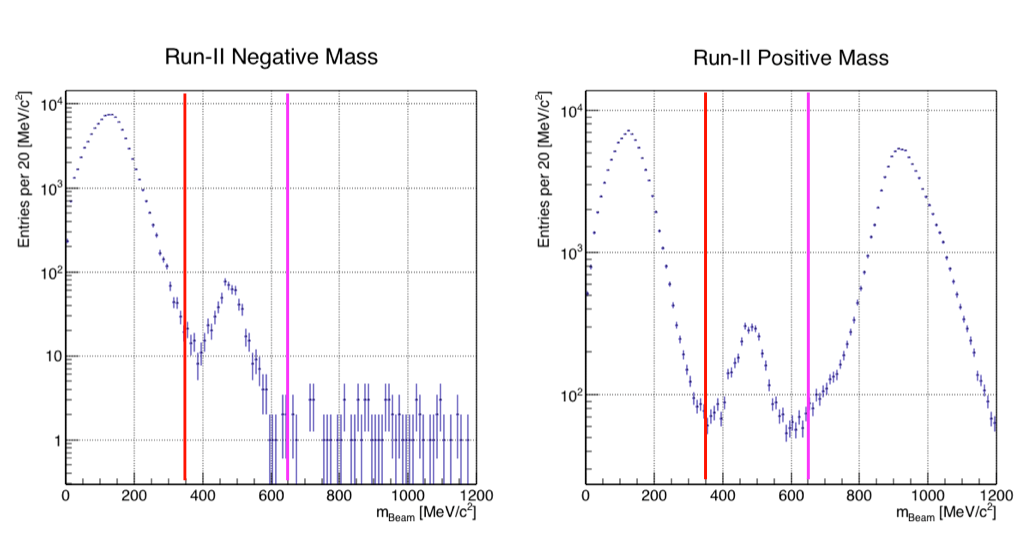
\includegraphics[width=\textwidth]{Chapter-4/Images/massRunII.png}
\caption{Distribution of the beamline mass as calculated according to equation \ref{eq:mass} for the Run-II events reconstructed in the beamline, negative polarity runs on the left and positive polarity runs on the right. The classification of the events into $\pi^\pm/ \mu^\pm/e^\pm$, K$^\pm$, or (anti)proton is based on these distributions, whose selection cut are represented by the vertical colored lines.}
\label{fig:mass}
\end{figure}

\subsection{TPC Selection: Halo Mitigation }\label{ch:pileUp}
The secondary beam impinging on LArIAT secondary target produces a plethora of particles which propagates downstream. The presence of upstream and downstream collimators greatly abates the number of particles tracing down the LArIAT tertiary beamline. However, it is possible that more than one particle sneaks into the LArTPC during its readout time: the TPC readout is triggered by the particle  firing the beamline detectors, but particles from the beam halo might be present in the TPC at the same time. We call ``pile up" the additional traces in the TPC. We adjusted the primary beam intensity between LArIAT Run I and Run II to reduce the presence of events with high pile up particles in the data sample. For the cross section analyses, we remove events with more than 4 tracks in the first 14 cm upstream portion of the TPC from the sample (line 6 in in Table \ref{tab:beamlineDataSelection}).


\subsection{TPC Selection: Shower Removal}\label{ch:electrons}
In the case of the ($\pi^-$,Ar) cross section, the resolution of  beamline mass spectrometer is not sufficient to select a beam of pure pions. In fact, muons and electrons survive the selection on the beamline mass. It is important to notice that the composition of the negative polarity beam is mostly pions, as will be discussed in section \ref{ch:beamlineComposition}.
Anyhow, we devise a selection on the TPC information to mitigate the presence of electrons in the sample used for the pion cross section. The selection relies on the different topologies of a pion and an electron event in the argon: while the former will trace a track inside the TPC active volume, the latter will tend to ``shower", i.e. interact with the medium, producing bremsstrahlung photons which pair convert into several short tracks. In order to remove the shower topology, we create a region of interest (ROI) around the TPC track corresponding to the beamline particle (more details on this in the next section). We look for short tracks contained in the ROI, as depicted in figure \ref{fig:showerFilt}:  if more then 5 tracks shorter than 10 cm are in the ROI, we reject the event. Line 8 in in Table \ref{tab:beamlineDataSelection}) shows the number of events surviving this selection.

\begin{figure}
  \centering  
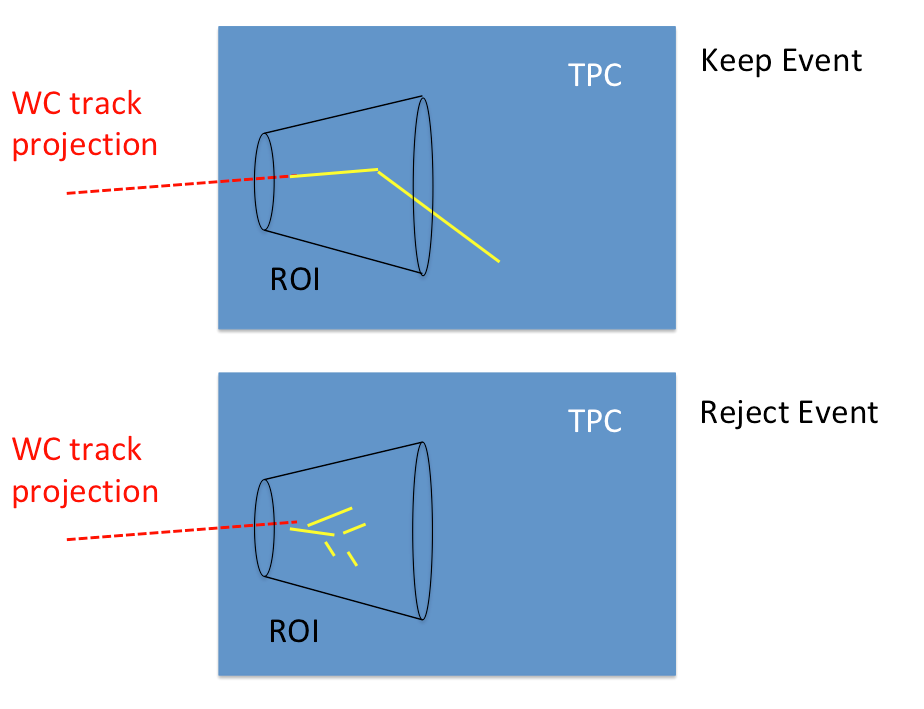
\includegraphics[width=\textwidth]{Chapter-4/Images/Shower.png}
\caption{Visual rendering of the shower filter. The ROI is a cut cone, with a small radius of 4 cm, a big radius of 10 cm and an height of 42 cm (corresponding to 3 radiation lengths for electrons in Argon).}
\label{fig:showerFilt}
\end{figure}



\section{Beamline and TPC Handshake: the Wire Chamber to TPC Match}\label{ch:WC2TPCMatchMethod}
For each event passing the selection on its beamline information, we need to identify the track inside the TPC corresponding to the particle which triggered the beamline detectors, a procedure we refer to as ``WC to TPC match" (WC2TPC for short). In general, the TPC tracking algorithm will reconstruct more than one track in the event, partially due to the fact that hadrons interact in the chamber and partially because of pile up particles during the triggered TPC readout time, as shown in figure~\ref{fig:kaonInteraction}. 


\begin{figure}
  \centering  
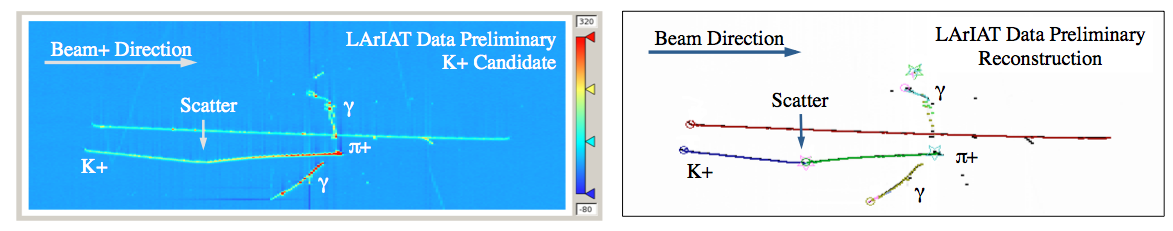
\includegraphics[width=\textwidth]{Chapter-4/Images/KaonExample.png}
\caption{Kaon candidate event: on the right, event display showing raw quantities; on the left, event display showing reconstructed tracks. In the reconstructed event display, different colors represent different track objects. A kink is visible in the kaon ionization, signature of a hadronic interaction: the tracking correctly stops at the kink position and two tracks are formed. An additional pile-up track is so present in the event (top track).}
\label{fig:kaonInteraction}
\end{figure}



We attempt to uniquely match one wire chamber track to one and only one reconstructed TPC track. 
In order to determine if the presence of a match, we apply a geometrical selection on the relative the position of the wire chamber and TPC tracks. 
We start by considering only TPC tracks whose first point is in the first 2 cm upstream portion of the TPC for the match.  We project the wire chamber track to the TPC front face where we define the coordinates of the projected point as  $x_{FF}$ and $y_{FF}$.  For each considered TPC track, we define $\Delta$X as the difference between the $x$ position of the most upstream point of the TPC track and $x_{FF}$.  $\Delta$Y is defined analogously. We define the radius difference, $\Delta$R, as $ \Delta \text{R} =  \sqrt{ \Delta \text{X}^2 +  \Delta \text{Y}^2}  $. We define  as $\alpha$ the angle between the incident WC track and the TPC track in the plane that contains them.  If  $\Delta \text{R} < 4 $~cm, $\alpha < 8^\circ $,  a match between WC-track and TPC reconstructed track is found. We describe  how we determine the value for the radius and angular selection in sec \ref{ch:WC2TPCMatchOptimization}.
In MC, we mimic the matching between the WC and the TPC track by constructing a fake WC track using truth information at wire chamber four. We then apply the same WC to TPC matching algorithm as in data. 
We discard events with multiple WC2TPC matches. We use only those TPC tracks that are matched to WC tracks in the cross section calculation.

\begin{figure}
  \centering  
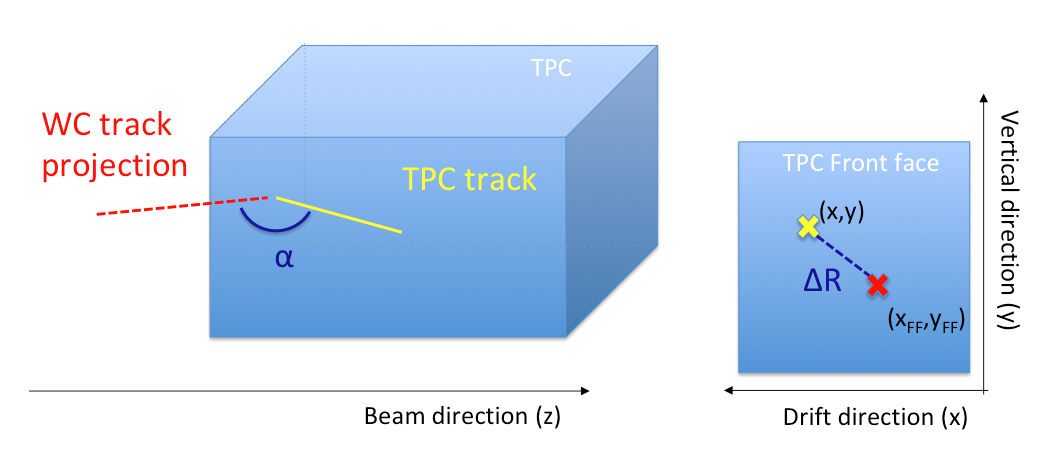
\includegraphics[width=\textwidth]{Chapter-4/Images/WC2TPCMatchTracks.png}
\caption{Visual rendering of the wire chamber to TPC match.}
\label{fig:showerFilt}
\end{figure}

\section{The Thin Slice Method}\label{ch:ThinSliceMethod}
Once we have selected the pool of hadron candidates and we have identified the TPC track corresponding to the beamline event, we apply the thin slice method to measure the cross section, as the following sections describe. 
\subsection{Cross Sections on Thin Target}
Cross section measurements on a thin target have been the bread and butter of nuclear and particle experimentalists since the Geiger-Marsden experiments \cite{Geiger1909}. At their core, these types of experiments consist in shooting a beam of particles with a known flux on a thin target and recording the outgoing flux. 


In general, the target is not a single particle, but rather a slab of material containing many diffusion centers. The so-called  ``thin target" approximation assumes that the target centers are uniformly distributed in the material and that the target is thin compared to the projectile interaction length,WC2TPC so that no center of interaction sits in front of another. In this approximation, the ratio between the number of particles interacting in the target $N_{Interacting}$ and number of incident particles $N_{Incident}$ determines the interaction probability $P_{Interacting}$, which is the complementary to one of the survival probability $P_{Survival}$. 
Equation \ref{eq:thinTargetXS} 
\begin{equation}
P_{Survival} = 1- P_{Interacting} = 1 - \frac{N_{Interacting}}{N_{Incident}} = e^{-\sigma_{TOT} n \delta X}
\label{eq:thinTargetXS}
\end{equation}
describes the probability for a particle to survive the thin target. This formula relates the total cross section $\sigma_{TOT}$, the density of the target centers  $n$  and  the thickness of the target  along the incident hadron direction $\delta X$, to the interaction probability\footnote{The scattering center density in the target, {\emph{n}},  relates to the argon density $\rho$, the Avogadro number  $ N_{A} $ and the argon molar mass $m_A$ as $n=\frac{\rho N_{A} }{m_A}$.}. If the target is thin compared to the interaction length of the process considered, we can Taylor expand the exponential function in equation \ref{eq:thinTargetXS} and find a simple proportionality relationship between the number of incident and interacting particles, and the cross section, as shown in equation \ref{eq:thinTargetXSTaylor}:
\begin{equation}
1 - \frac{N_{Interacting}}{N_{Incident}} =  1 -\sigma_{TOT} n \delta X + O(\delta X^2).
\label{eq:thinTargetXSTaylor}
\end{equation}

Solving for the cross section, we find:
\begin{equation}
 \sigma_{TOT}  = \frac{1}{n \delta X}\frac{N_{Interacting}}{N_{Incident}}.
\label{eq:thinTargetXSSolved}
\end{equation}

\subsection{Not-so-Thin Target: Slicing the Argon}\label{ch:XSRaw}
The interaction length of pions and kaons in argon is expected to be of the order of 50 cm for pions and 100 cm for kaons. Thus, the LArIAT TPC, with its 90 cm of length, is not a thin target. However, the fine-grained tracking of the LArIAT LArTPC allows us to treat the argon volume as a sequence of many adjacent thin targets. 

As described in Chapter \ref{sec:experimentDescription}, LArIAT wire planes consist of 240 wires each. The wires are oriented at +/- $60^{\circ}$ from the vertical direction at 4 mm spacing, while the beam direction is oriented 3 degrees off the $z$ axis in the $XZ$ plane.  The wires collect signals proportional to the energy loss of the hadron along its path in a  $\delta${\emph{X}} = 4 mm/sin($60^{\circ}$) $\approx$ 4.7~mm slab of liquid argon. Thus, one can think to slice the TPC into many thin targets of $\delta${\emph{X}} = 4.7~mm thickness along the direction of the incident particle, making a measurement at each wire along the path.

Considering each slice {\emph{j}}  a ``thin target",  we can apply the cross section calculation from Equation~\ref{eq:thinTargetXSSolved} iteratively, evaluating the kinetic energy of the hadron as it enters each slice, $E_{j}^{kin}$.  For each WC2TPC matched particle, the energy of the hadron entering the TPC is known thanks to the momentum and mass determination by the tertiary beamline, 

\begin{equation}
 E^{kin}_{Front Face}  = \sqrt{p^2_{Beam} - m^2_{Beam}} - m_{Beam} - E_{loss},
\label{eq:enFF}
\end{equation}
where $E_{loss}$ is a correction for the energy loss in the dead material between the beamline and the TPC front face. The  energy of the hadron at each slab is determined by subtracting the energy released by the particle in the previous slabs. For example, at the $j^{th}$ point of a track, the kinetic energy will be

\begin{equation}
 E_{j}^{kin} =  E^{kin}_{Front Face} - \sum_{i < j} \Delta E_i,
\label{eq:KEj}
\end{equation}
where $\Delta E_i$ is the energy deposited at each argon slice before the $j^{th}$ point as measured by the calorimetry associated with the tracking.


If the particle enters a slice, it contributes to $N_{Incident}( E^{kin})$ in the energy bin corresponding to its kinetic energy in that slice. If it interacts in the slice, it then also contributes to $N_{Interacting}(E^{kin})$ in the appropriate energy bin. The cross section as a function of kinetic energy, $\sigma_{TOT}( E^{kin})$ will then be proportional to the ratio $\frac{N_{Interacting}( E^{kin})}{N_{Incident}( E^{kin})}$ .






\subsection{Corrections to the Raw Cross Section}\label{ch:MCCorrections}
%%%%%%%%%%%%%%%%%%%%%%%%%%
Equation \ref{eq:thinTargetXSSolved}  is a prescription for measuring the cross section in case of a pure beam of the hadron of interest and 100\% efficiency in the determination of the interaction point.  For example, if LArIAT had a beam of pure pions and were 100\% efficient in determining the interaction point within the TPC, the pion cross section in each energy bin would be given by

\begin{equation}
 \sigma^{\pi^-}(E_{i})  = \frac{1}{n \delta X}\frac{N^{\pi^-}_{ \text{Interacting}} (E_{i})}{N^{\pi^-}_{ \text{Incident}}(E_{i})}.
\label{eq:thinTargetXSSolved2}
\end{equation}

Unfortunately, this is not the case. In fact, the selection used to isolate pions in the LArIAT beam allows for the presence of some muons and electrons as background. Also, the LArIAT TPC is not 100\% efficient in determining the interaction point. Therefore we need to apply two corrections evaluated on the MC in order to extract the cross section from LArIAT data: the background subtraction and the efficiency correction. 
Still using the pion case as example, we estimate the pion cross section in each energy bin changing  Equation \ref{eq:thinTargetXSSolved2} into
\begin{equation}
 \sigma^{\pi^-}(E_{i})  =\frac{1}{n \delta X}\frac{N^{\pi^-}_{ \text{Interacting}} (E_{i})}{N^{\pi^-}_{ \text{Incident}}(E_{i})} = \frac{1}{n \delta X}\frac{ \epsilon^{inc}_i [ N^{ \text{TOT}}_{ \text{Interacting}} (E_{i}) - B_{ \text{Interacting}} (E_i)] }{   \epsilon^{int}_i [N^{ \text{TOT}}_{ \text{Incident}}(E_{i}) - B_{ \text{Incident}} (E_i)]},
\label{eq:True}
\end{equation}



 
where  $N^{\text{TOT}}_{\text{Interacting}} (E_{i})$ and $N^{\text{TOT}}_{\text{Incident}} (E_{i})$ is the measured content of the interacting and incident histograms for events that pass the event selection, $B_{interacting} (E_i)$ and $B_{\text{Incident}} (E_i)$ represent the contributions from beamline background, and  $\epsilon^{int}_i$ and  $\epsilon^{inc}_i$ are the efficiency corrections for said histograms. 

As we will show in section \ref{sec:Correction}, the background subtraction for the interacting and incident histograms can be translated into a corresponding corrections $C^{\pi MC}_{Interacting} (E_{i})$ and $C^{\pi MC}_{Incident} (E_{i})$ and the cross section re-written as follows

\begin{equation}
      \sigma^{\pi^-}(E_{i})  = \frac{1}{n \delta X}\frac{ \epsilon^{\text{Inc}}(E_i)  \hspace{0.2cm} C^{\pi MC}_{\text{Int}} (E_{i}) \hspace{0.2cm} N^{\text{TOT}}_{\text{Int}} (E_{i}) }{   \epsilon^{\text{Int}}(E_i) \hspace{0.2cm} C^{\pi MC}_{\text{Inc}} (E_{i}) \hspace{0.2cm}  N^{\text{TOT}}_{\text{Inc}} (E_{i})}.
\label{eq:C}
\end{equation}



%The following sections describe the procedures used to evaluate  the background subtraction (section \ref{sec:beamCont}) and the efficiency correction (section \ref{sec:EffCorrection}), as well as  their uncertainties. 
%The reader might be concerned about bin-by-bin migration of events in the interacting and incident plots due to the finite resolution of the energy reconstruction. In section \ref{sec:Energy}, we make an argument to why we expect the smearing matrix to be extremely close to diagonal, such that its calculation and relative corrections are left for an improvement of the analysis.


%%%%%%%%%%%%%%%%%%%%%%%%%%%%%%%%%%%%%%%%%%%%%%%%



\section{Procedure testing with truth quantities}\label{ch:procedureTesting}
The ($\pi^{-}$,Ar) and (K$^{+}$,Ar) total hadronic cross section implemented in Geant4 can be used as a tool to validate the measurement methodology.  We describe here a closure test done on Monte Carlo to prove that the methodology of slicing the TPC retrieves the underlying cross section distribution implemented in Geant4 within the statistical uncertainty. %under the working assumption of perfect reconstruction.

For pions in the considered energy range, \textcolor{red}{the Geant4 inelastic model adopted to is ``BertiniCascade", while the elastic model ``hElasticLHEP".}
For kaons, the Geant4 inelastic model adopted to is ``BertiniCascade", while the elastic model ``hElasticLHEP".  


For the validation test, we fire about a sample of pions and a sample of kaons inside the LArIAT TPC active volume using the Data Driven Monte Carlo (see section \ref{sec:DDMC}). We apply  the thin-sliced method using only true quantities to calculate the hadron kinetic energy at each slab in order to decouple reconstruction effects from issues with the methodology.  For each slab of 4.7 mm length along the path of the hadron, we integrate the true energy deposition as given by the Geant4 transportation model. Then, we recursively subtracted it from the hadron kinetic energy at the TPC front face to evaluate the kinetic energy at each slab until the true interaction point is reached. Since the MC is a pure beam of the hadron of interest and truth information is used to retrieve the interaction point, no correction is applied. Doing so, we obtain the true interacting and incident distributions for the considered hadron and we obtain the true MC cross section as a function of the hadron true kinetic energy. 

Figure \ref{fig:TrueMCXS2} shows the total hadronic cross section for argon implemented in Geant4 10.01.p3 (solid lines) overlaid with the true MC cross section as obtained with the sliced TPC method (markers) for pions on the left and kaons on the right; the total cross section is shown in green,  the elastic cross section in blue and the inelastic cross section in red.  The nice agreement with the Geant4 distribution and the cross section  obtained with the sliced TPC method gives us confidence in the  validity of the methodology. 
        
%\begin{comment}     
\begin{figure}
%\captionsetup{justification=raggedright}  
\begin{minipage}[b]{.53\textwidth}  
  \centering  
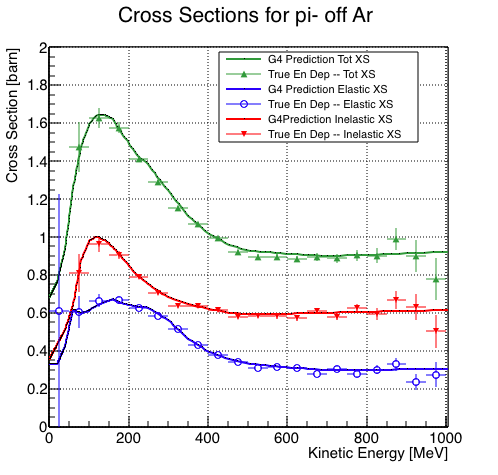
\includegraphics[width=3in]{Chapter-4/Images/PionTrueXS.png}
\end{minipage}%  
\begin{minipage}[b]{0.53\textwidth}  
  \centering  
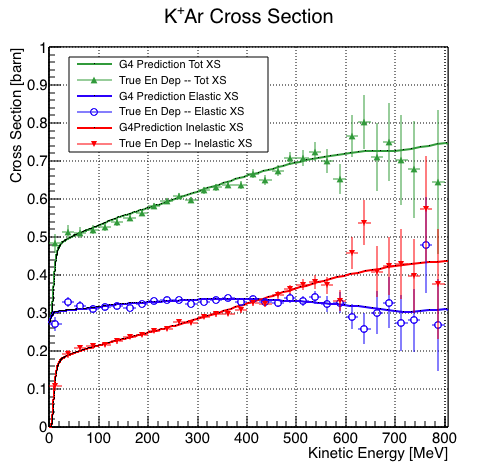
\includegraphics[width=3in]{Chapter-4/Images/KaonTrueXS.png}
\end{minipage}
\caption{Hadronic cross sections for ($\pi^-$,Ar) on the left and (K$^+$,Ar) on the right as implemented in Geant4 10.01.p3 (solid lines) overlaid the true MC cross section as obtained with the sliced TPC method (markers). The total cross section is shown in green,  the elastic cross section in blue and the inelastic cross section in red.}
\label{fig:TrueMCXS2}
\end{figure}
%\end{comment}





